\documentclass{beamer}

\mode<presentation>
{
  \usetheme{Warsaw}

  \setbeamercovered{transparent}
}


\usepackage[english]{babel}

\usepackage{graphicx}

\usepackage{amsmath}
\usepackage{algorithm,algorithmic}
\usepackage[utf8]{inputenc}

\usepackage{times}
\usepackage[T1]{fontenc}
\newcommand{\kmeans}{$k$-means}
\makeatletter
\renewcommand*{\ALG@name}{Algoritme}
\makeatother
\title{Clusteringsalgoritmen}

\subtitle{Bachelorproef}

\author{Victor Miclotte}

\institute{Universiteit Gent}

\date{26 mei 2016}

\subject{Bachelorproef}
	

%%%%%%%%%%%%%%%%%%%%%%%%%%%%%%%%%%%%%%%%%%%%%%

\begin{document}
	\titlepage
	\begin{figure}
	\centering
	\includegraphics[scale = 0.25]{logo} 
	\end{figure}

	
\begin{frame}{Inhoud}
	\tableofcontents
\end{frame}

\section{Motivatie}


\begin{frame}{Motivatie}
Veel toepassingen in verschillende takken van de wetenschap.
\begin{itemize}
 \item Biologie: genexpressies
 \item Economie: prijsfluctuaties
 \item Taalkunde: teksten vergelijken
 \item \ldots
\end{itemize}
\end{frame}


\section{\kmeans}


\begin{frame}{\kmeans}
\begin{itemize}
 \item Partitioneel clusteringsalgoritme
 \item Elke cluster wordt geassocieerd met een center
 \item $k$ op voorhand vastgelegd
\end{itemize}

\begin{algorithm}[H]
\begin{algorithmic}[1]
\STATE Selecteer $k$ punten als initiële centers.
\WHILE{centers zijn veranderd}
\STATE Voeg elk punt toe aan cluster met dichtste center.
\STATE Herbereken centers van elke cluster.
\ENDWHILE
\end{algorithmic}
\caption{\kmeans}
\end{algorithm}
\end{frame}

\begin{frame}{\kmeans:\ voorbeeld}
 \begin{figure}[!ht]\centering
  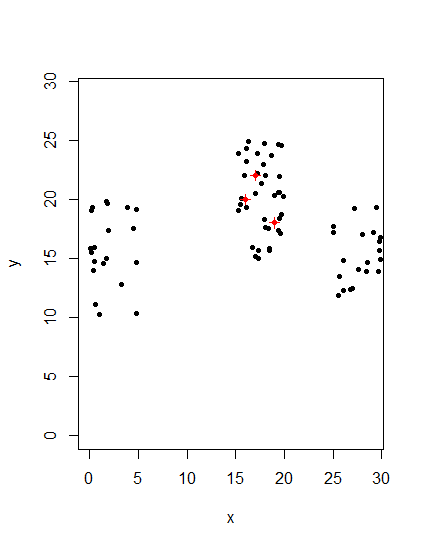
\includegraphics[width=5.2cm]{kmeans.png}
 \end{figure}
\end{frame}

\begin{frame}{\kmeans:\ voorbeeld}
 \begin{figure}[!ht]\centering
  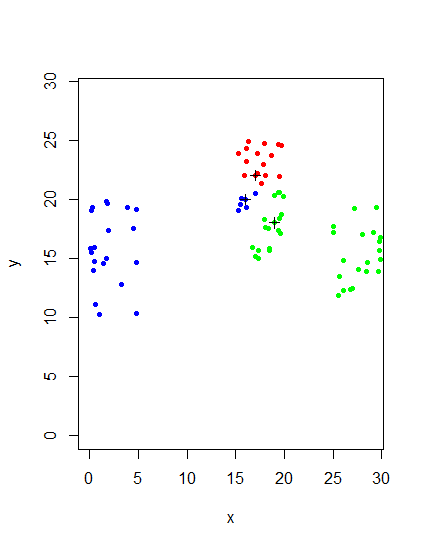
\includegraphics[width=5.2cm]{kmeans_it0.png}
 \end{figure}
\end{frame}

\begin{frame}{\kmeans:\ voorbeeld}
 \begin{figure}[!ht]\centering
  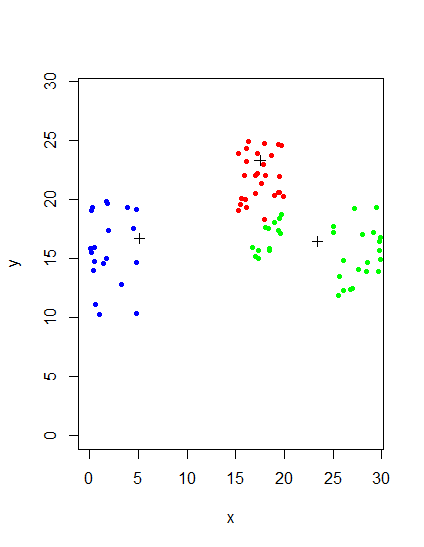
\includegraphics[width=5.2cm]{kmeans_it1.png}
 \end{figure}
\end{frame}

\begin{frame}{\kmeans:\ voorbeeld}
 \begin{figure}[!ht]\centering
  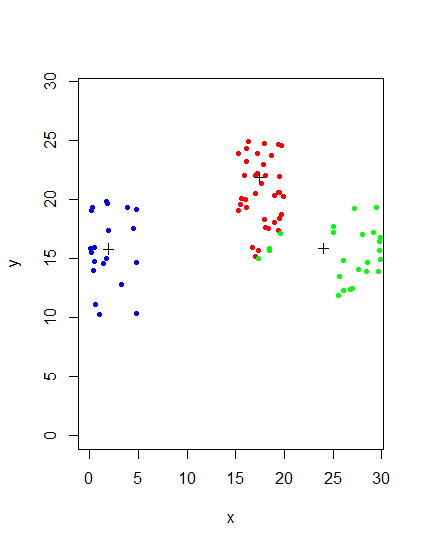
\includegraphics[width=5.2cm]{kmeans_it2.png}
 \end{figure}
\end{frame}

\begin{frame}{\kmeans:\ voorbeeld}
 \begin{figure}[!ht]\centering
  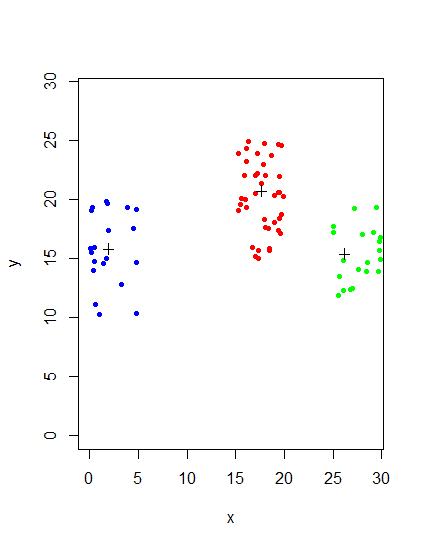
\includegraphics[width=5.2cm]{kmeans_it3.png}
 \end{figure}
\end{frame}

\begin{frame}{\kmeans:\ voorbeeld}
 \begin{figure}[!ht]\centering
  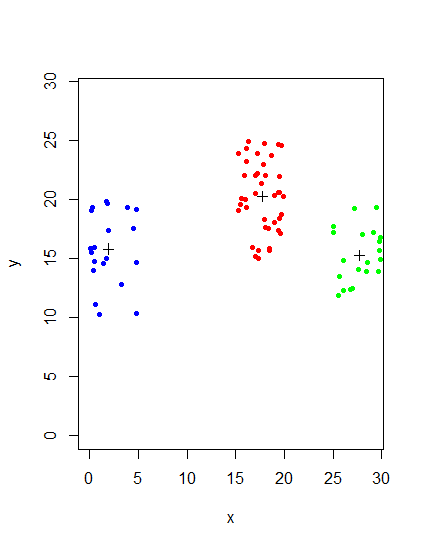
\includegraphics[width=5.2cm]{kmeans_it4.png}
 \end{figure}
\end{frame}

\begin{frame}{Initiële centers}
 \begin{figure}[!ht]\centering
  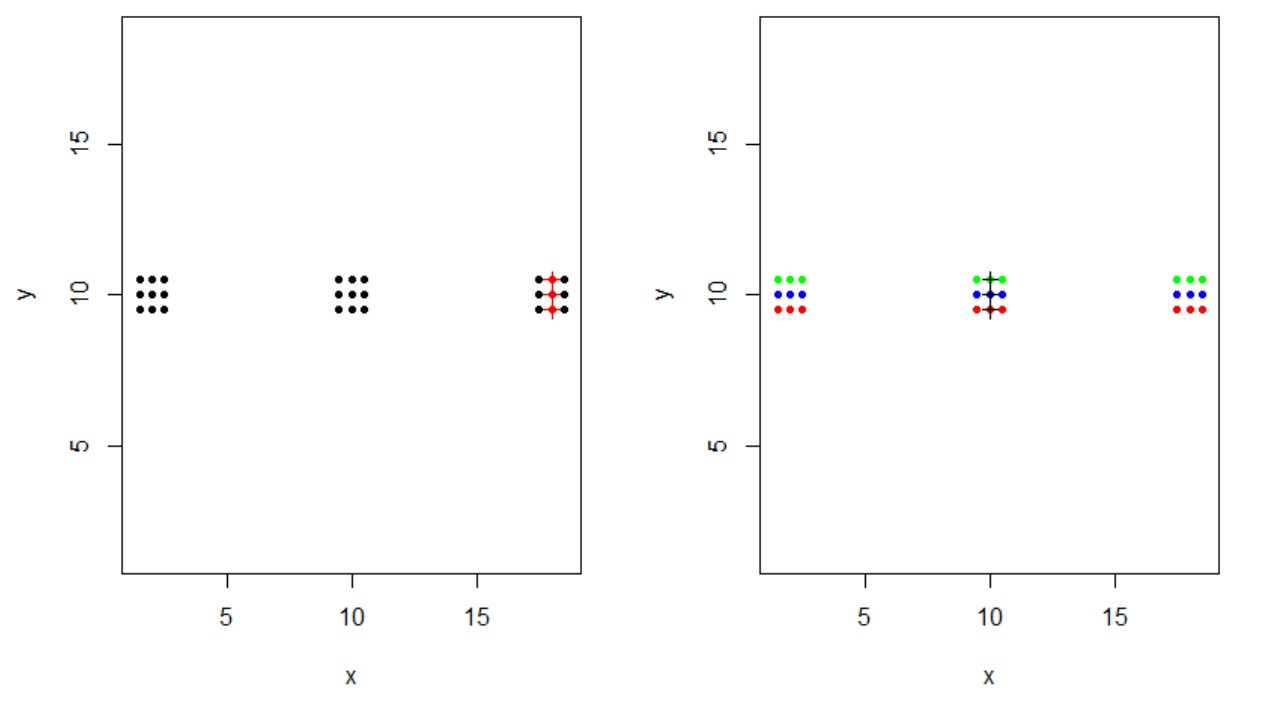
\includegraphics[width=11cm]{kmeans_bad.jpeg}
 \end{figure}
\end{frame}

\begin{frame}{Andere problemen}
 \begin{itemize}
  \item Lege clusters
  \item Niet-sferische clusters
  \item Clusters zijn in elkaar verweven
 \end{itemize}

 \begin{figure}[!ht]\centering
  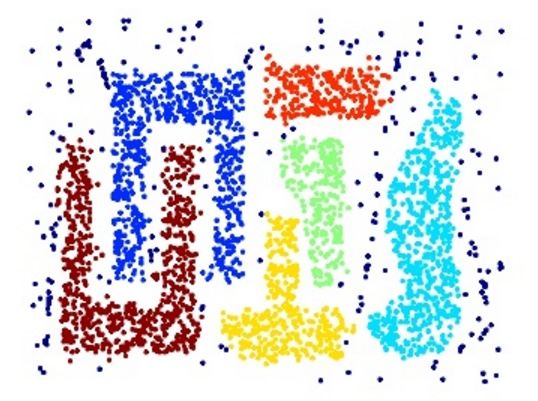
\includegraphics[width=5.2cm]{dbscan_nonspheric.jpg}
 \end{figure}
\end{frame}

\begin{frame}{Uitbreidingen}
 \begin{itemize}
  \item Pre-processing
  \item Post-processing: verlagen van de SSE
  \item Bisecting \kmeans
 \end{itemize}
\end{frame}

\begin{frame}{Post-processing: verlagen van de SSE}
 Twee fasen:
 \begin{itemize}
  \item Aantal clusters verhogen en SSE verlagen
  \item Clusters samenvoegen waarbij SSE zo weinig mogelijk stijgt
 \end{itemize}
\end{frame}

\section{Hiërarchisch clusteren}
\begin{frame}{Hiërarchisch clusteren}
 \begin{itemize}
  \item Sequentie van partitionele clusteringen
  \item Afstandsmatrix
  \item Single link / Complete link / Group average
 \end{itemize}
\begin{algorithm}[H]
\textbf{Input:} een $n\times n$-afstandsmatrix.\\
\begin{algorithmic}[1]
\STATE Maak $n$ clusters met elk één punt.
\WHILE{Er is meer dan één cluster}
\STATE Voeg de twee dichtste clusters samen.
\STATE{Pas de afstandsmatrix aan.}
\ENDWHILE
\end{algorithmic}
\caption{Hiërarchisch clusteren}
\end{algorithm}
\end{frame}

\begin{frame}{Dendrogram}
 \begin{figure}[!ht]\centering
  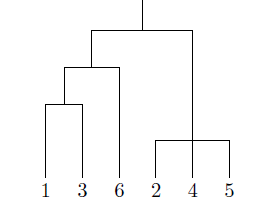
\includegraphics[width=5.2cm]{dendrogram.png}
 \end{figure}
\end{frame}


\section{DBScan}
\begin{frame}{DBScan}
 Densiteit (= aantal punten binnen bepaalde straal $\epsilon$) i.p.v.
 afstanden gebruiken om clusters te vormen.
 \begin{itemize}
  \item $MinPts$: density-treshold
  \item \textbf{Kernpunt:} punt met dichtheid $\geq MinPts$
  \item \textbf{Randpunt:} punt in omgeving van kernpunt
  \item \textbf{Ruispunt:} elk ander punt
 \end{itemize}

\end{frame}

\begin{frame}
 Bepalen van $MinPts$ en $\epsilon$
 \begin{figure}[!ht]\centering
  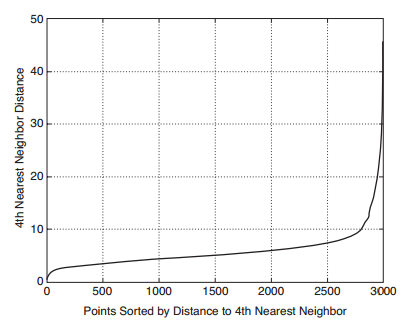
\includegraphics[width=8cm]{dbscan_kdist.png}
 \end{figure}

\end{frame}
 
 
 
\begin{frame}
 Clusters met verschillende densiteit
 \begin{figure}[!ht]\centering
  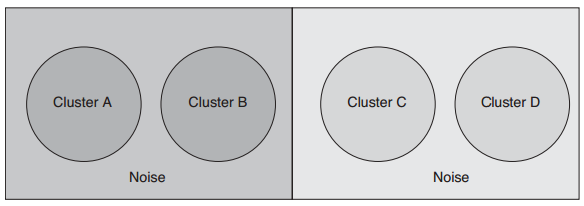
\includegraphics[width=11cm]{dbscan_density.png}
 \end{figure}

\end{frame}

\section{Clusterevaluatie}
\begin{frame}{Clusterevaluatie}
 \begin{itemize}
  \item Kwaliteit nagaan: cohesie en separatie
  \item Aantal clusters bepalen
  \item Geschikt voor clustering
 \end{itemize}

\end{frame}


\end{document}
